\documentclass{thureport}
% =============================================
% Part 1 Edit the info
% =============================================

\newcommand{\major}{软件71}
\newcommand{\name}{骆炳君}
\newcommand{\stuid}{2017013573}
\newcommand{\newdate}{2019-5-13}
\newcommand{\newtitle}{同轴电缆中电磁波的传输与金属中超声波的传输}
\newcommand{\dL}{\delta L}
\def\celsius{{\ensuremath{^\circ\hspace{-0.09em}\mathrm{C}}}}

% =============================================
% Part 1 Main document
% =============================================
\begin{document}
\thispagestyle{empty}
\begin{figure}[h]
	\begin{minipage}{0.65\linewidth}
		\centerline{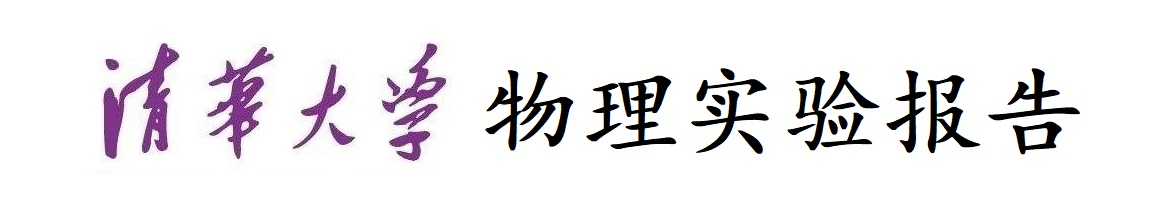
\includegraphics[width=\linewidth]{head.jpg}}
	\end{minipage}
	\hfill
	\begin{minipage}{.3\linewidth}
		\raggedleft
		\begin{tabular*}{.8\linewidth}{ll}
			班级: & \underline\major   \\
			姓名: & \underline\name    \\
			学号: & \underline\stuid   \\
			日期: & \underline\newdate
		\end{tabular*}
	\end{minipage}
\end{figure}
 
\begin{table}[!htbp]
	\centering\large
	实验名称: \underline\newtitle
\end{table}

\tableofcontents
% =============================================
% Part 2 Main document
% =============================================
\newpage

\section{实验目的}
\begin{clause}
	\item 学习掌握脉冲波信号的测量方法.
	\item 学习理解波遇到界面时的反射和透射特性,入射波与反射波的相位关系.
	\item 学习掌握超声波波速的测量方法,观察声波转换和表面波.
	\item 学习了解超声波探伤的原理.
\end{clause}

\section{实验原理}
\subsection{同轴电缆中电磁波的测量和应用}
电磁波在同轴电缆的中心导体和屏蔽层之间传输,是一封闭电路. 高频信号具有集肤效应,电流只在中心导体的表面流动,因此电磁场与外界不会相互干扰,具有良好的屏蔽性.

传输线为一对相隔均匀距离的平行导线或同轴电缆线,其上的电信号存在随长度变化的空间分布,负载不匹配时还会有驻波分布.

在上图中,$R,L,C,G$分别为单位长度传输线的电阻、电感、电容和电导,$v(z,t)$和$i(z,t)$为沿传输线方向的电压和电流信号. 利用电路方程分析单元传输线可得微分方程

$$\frac{d^2V(z)}{dz^2}=\gamma^2V(z),\ \frac{d^2I(z)}{dz^2}=\gamma^2I(z)$$

其中$\gamma=\alpha+j\beta=\sqrt{(R+j\omega L)(G+j\omega C)}$,$\alpha$和$\beta$都是和$\omega$相关的伪常数. 由微分方程的解和两端的边界条件可得,在线上任意一点处都有

$$V(z)=\frac{I_l}{2}(Z_l+Z_0)e^{\gamma(l-z)}(1+\Gamma e^{-2\gamma(l-z)})$$

其中$\Gamma=\frac{Z_l-Z_0}{Z_l+Z_0}$,是在负载端电压反射波与入射波振幅之比,称为负载$Z_l$的电压反射系数. 若负载$Z_l$是纯电阻性负载,分以下三种情况:

\subparagraph{开路时}$Z_l=R_l=\infty$,$\Gamma=1$. 电压反射系数最大,在$z=l$处,电压最大,电流最小.

\subparagraph{短路时}$Z_l=R_l=0$,$\Gamma=-1$. 电压反射系数为负,反射波为反相,电压、电流驻波分布与开路情况相反.

\subparagraph{负载匹配时}$Z_l=R_l=R_0$,$\Gamma=0$. 电压反射系数为0,此时没有反射波,线路中只有沿$+z$方向的行波.

\subsection{金属中超声波的传输}
超声波在介质中传播有纵波、横波和表面波三种形式. 当超声纵波或横波入射到介质1与介质2界面上时,若介质都是固体或其中之一是固体,在发生反射和折射时,一般会同时反射或折射出另一种波形,超声波的这种特性被称为波形转换. 设$\theta$为介质1中的入射角,$c_1$为介质1中的波速,$c_{2l},c_{2s}$为介质2中纵波和横波的波速,$\beta_s,\beta_l$分别为介质2中纵波和横波的折射角,根据折射定律有

$$\frac{\sin\theta}{c_1}=\frac{\sin\beta_l}{c_{2l}}=\frac{\sin\beta_s}{c_{2s}}$$

在超声波分析测试中,利用超声波探头产生脉冲超声波,常用的超声波探头有直探头、斜探头和可变角探头. 实验中使用的探头工作方式主要为单探头方式,即同一个探头,既用来发射超声,又用来接受超声.

\section{实验仪器}
\begin{clause}
	\item 数字示波器
	\item 信号发生器
	\item 超声波测试仪
	\item 电阻盒、待测长同轴电缆、短同轴电缆连接线、三通接头、阻抗元件等
\end{clause}

\section{实验步骤}
\subsection{测量同轴电缆的长度和衰减常数}
\begin{figure}[H]
	\centering
	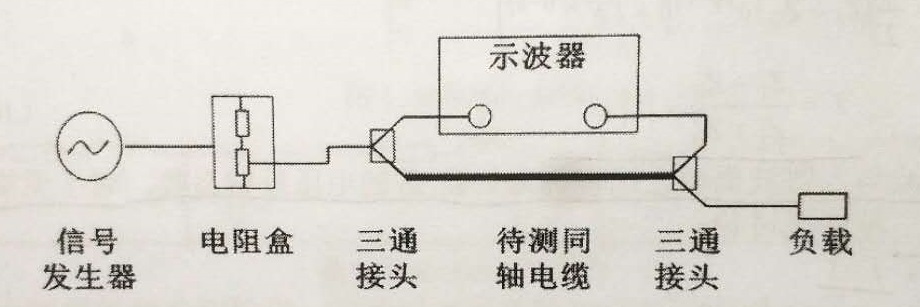
\includegraphics[width=0.5\linewidth]{figure1.jpg}
\end{figure}

根据上图所示的电路连接实验电路,信号发生器选择$40$kHz左右的连续脉冲,信号峰值在2至5V之间,占空比约为$0.5\%$,传输线负载端分别选择开路、短路和匹配电阻三种测试方式,利用示波器分别测出输入端和负载端之间的信号波形和相对延时. 开路负载时,计算电缆长度和吸收系数$\alpha$,短路负载时,计算延时并重复测量3次,匹配负载时,计算延时并重复测量3次. 分别利用测量结果计算同轴电缆的长度,并估算不确定度.

\subsection{超声波测量}
\subparagraph{利用直探头测量纵波声速$c_l$}
把直探头置于试样上表面,用示波器显示试样底面的反射回波,反复移动探头直至回波信号最大,测量起始波与回波的时间$t_1,t_2$.

\subparagraph{利用$45^\circ$斜探头测量横波声速$c_s$}
把$45^\circ$斜探头置于试样弧形部分的圆心位置,用示波器显示圆弧边界发射回波,移动探头使回波信号达到最大值,测量回波时间$t_1,t_2$.

\subparagraph{利用可变角探头测量表面波声速$c_b$}
将可变角探头的角度调至$65^\circ$左右,采用移动法,先找出起始点的反射回波在示波器时间轴的位置,沿传播方向移动探头,再找出反射回波的第二个位置,测量两者的距离和时间差.

\subsection{超声波探伤}
\subparagraph{直探头测量缺陷C的深度}
将直探头置于缺陷C的正上方,确定反射波和缺陷波的位置,测量两者的时间差.

\subparagraph{斜探头测量缺陷D的深度}
移动斜探头使其对正缺陷A和B,测量回波时间$t_A,t_B$和水平距离$x_A,x_B$,确定探头的参数. 再测量缺陷D的回波时间$t_D$和水平距离$x_D$.

\section{数据处理}
\subsection{同轴电缆的长度和衰减系数}
已知电磁波在该电缆中波速$u=2.0\times10^8m/s$,仪器误差$\Delta B=10ns$.

\subsubsection{开路负载测量长度和吸收系数}
使用逐差法计算时间差
$$\delta t_1=\frac{\tau_4-\tau_1}{3}=114.7ns,\ \delta t_2=\frac{\tau_5-\tau_2}{3}=117.3ns,\ \delta t_3=\frac{\tau_6-\tau_3}{3}=117.3ns$$

$$\delta t=\frac{\delta t_1+\delta t_2+\delta t_3}{3}=116.4ns$$

电缆长度
$$l=u\delta t=23.3m$$

$\delta t$的标准偏差
$$S_{\delta t}=\sqrt{\frac{1}{3\times(3-1)}\sum_{i=1}^3(\delta t_i-\delta t)^2}=0.87ns$$

$\delta t$的不确定度
$$\Delta_{\delta t}=\sqrt{\Delta_A^2+\Delta_B^2}=\sqrt{(t_p(2)S_{\delta t})^2+\Delta_B^2}=10.68ns$$

$l$的不确定度
$$\Delta_l=u\Delta_{\delta t}=2.1m$$

所以电缆长度的测量结果为$(23.3\pm 2.1)m$.

由公式
$$\alpha=\frac{\ln(V/V_l)}{l}$$

使用逐差法得吸收系数
$$\alpha=\frac{\ln(V_1V_2V_3)-\ln(V_4V_5V_6)}{9l}=0.0078m^{-1}$$

\subsubsection{短路负载测量长度}
$$\delta t_1=\tau_4-\tau_2=212ns,\ \delta t_2=\tau_6-\tau_4=216ns$$

时间差
$$\delta t=\frac{\delta t_1+\delta t_2}{2}=214ns$$

电缆长度
$$l=u\delta t/2=21.4m$$

$\delta t$的标准偏差
$$S_{\delta t}=\sqrt{\frac{1}{2\times(2-1)}\sum_{i=1}^2(\delta t_i-\delta t)^2}=2ns$$

$\delta t$的不确定度
$$\Delta_{\delta t}=\sqrt{\Delta_A^2+\Delta_B^2}=\sqrt{(t_p(1)S_{\delta t})^2+\Delta_B^2}=27.32ns$$

$l$的不确定度
$$\Delta_l=u\Delta_{\delta t}/2=2.7m$$

所以电缆长度的测量结果为$(21.4\pm 2.7)m$.

\subsubsection{匹配负载测量长度}
时间差
$$\delta t=\frac{\tau_1+\tau_2+\tau_3}{3}=96.0ns$$

电缆长度
$$l=u\delta t=19.2m$$

$\delta t$的标准偏差
$$S_{\delta t}=\sqrt{\frac{1}{3\times(3-1)}\sum_{i=1}^3(\tau_i-\delta t)^2}=2.31ns$$

$\delta t$的不确定度
$$\Delta_{\delta t}=\sqrt{\Delta_A^2+\Delta_B^2}=\sqrt{(t_p(2)S_{\delta t})^2+\Delta_B^2}=14.09ns$$

$l$的不确定度
$$\Delta_l=u\Delta_{\delta t}=2.8m$$

所以电缆长度的测量结果为$(19.2\pm 2.8)m$.

\subsection{超声波声速和杨氏模量}
已知示波器误差$\Delta_B=1\mu s$,$R_1=30.00mm$,$R_2=H=60.10mm$,$\Delta_H=\Delta_D=\Delta_{R_1}=\Delta_{R_2}=0.02mm$,$\rho=2.7\times10^kg\cdot m^{-3}$,$\Delta L=0.5mm$.

\subsubsection{测量纵波声速$c_l$}
时间差
$$\delta t=\frac{\delta t_1+\delta t_2+\delta t_3}{3}=19.73\mu s$$

纵波声速
$$c_l=\frac{2H}{\delta t}=6.092\times10^3m/s$$

$\delta t$的标准偏差$S_{\delta t}=0.133\mu s$.

$\delta t$的不确定度
$$\Delta_{\delta t}=\sqrt{\Delta_A^2+\Delta_B^2}=\sqrt{(t_p(2)S_{\delta t})^2+\Delta_B^2}=1.15\mu s$$

$c_l$的不确定度
$$\Delta_{c_l}=\sqrt{(\frac{2H}{\delta t^2}\Delta_{\delta t})^2+(\frac{2}{\delta t}\Delta_H)^2}=355m/s$$

所以纵波声速的测量结果为$(6.09\pm0.36)\times10^3m/s$.

\subsubsection{测量横波声速$c_s$}
时间差
$$\delta t=\frac{\delta t_1+\delta t_2+\delta t_3}{3}=19.33\mu s$$

横波声速
$$c_s=\frac{2(R_2-R_1)}{\delta t}=3.11\times10^3m/s$$

$\delta t$的标准偏差$S_{\delta t}=0.133\mu s$.

$\delta t$的不确定度
$$\Delta_{\delta t}=\sqrt{\Delta_A^2+\Delta_B^2}=\sqrt{(t_p(2)S_{\delta t})^2+\Delta_B^2}=1.15\mu s$$

$c_s$的不确定度
$$\Delta_{c_s}=\sqrt{(\frac{2(R_2-R_1)}{\delta t^2}\Delta_{\delta t})^2+(\frac{2\sqrt{2}}{\delta t}\Delta_{R_1})^2}=185m/s$$

所以横波声速的测量结果为$(3.11\pm0.19)\times10^3m/s$.

\subsubsection{测量表面波声速$c_b$}
计算得到3组声速数据
$$c_1=\frac{2L_1}{\delta t_1}=2941m/s,\ c_2=\frac{2L_2}{\delta t_2}=2885m/s, c_3=\frac{2L_3}{\delta t_3}=2907m/s$$

表面波声速
$$c_b=\frac{c_1+c_2+c_3}{3}=2.91\times10^3m/s$$

$c_1$的不确定度
$$\Delta_{c_1}=\sqrt{(\frac{2L_1}{\delta t_1^2}\Delta_{\delta t})^2+(\frac{2}{\delta t_1}\Delta_L)^2}=457m/s$$

$c_2$的不确定度
$$\Delta_{c_2}=\sqrt{(\frac{2L_2}{\delta t_2^2}\Delta_{\delta t})^2+(\frac{2}{\delta t_2}\Delta_L)^2}=294m/s$$

$c_3$的不确定度
$$\Delta_{c_3}=\sqrt{(\frac{2L_3}{\delta t_3^2}\Delta_{\delta t})^2+(\frac{2}{\delta t_3}\Delta_L)^2}=179m/s$$

$c$的不确定度
$$\Delta_c=\frac{\sqrt{\Delta_{c_1}^2+\Delta_{c_3}^2+\Delta_{c_3}^2}}{3}=191m/s$$

所以表面波声速的测量结果为$(2.91\pm0.19)\times10^3m/s$.

\subsubsection{测量杨氏模量$E$和Poisson系数$\sigma$}
$$T=\frac{c_l}{c_s}=1.96$$

杨氏模量
$$E=\frac{\rho c_s^2(3T^2-4)}{T^2-1}=69.15GPa$$

Poisson系数
$$\sigma=\frac{T^2-2}{2(T^2-1)}=0.324$$

\subsection{超声波探伤}
\subsubsection{直探头测量缺陷C的深度}
缺陷C的深度
$$H_c=H-\frac{H(t_q-t_l)}{t_H-t_l}=13.63mm$$

\subsubsection{斜探头测量缺陷D的位置}
已知$L_A=20mm$,$L_B=50mm$,$H_A=20mm$,$H_B=10mm$.

设斜探头的延迟为$t_0$,入射点距其右边缘的距离为$X_0$.

由
$$\sin\beta=\frac{X_0+X_A-L_A}{c(t_A-t_0)}=\frac{X_0+X_B-L_B}{c(t_B-t_0)}=\frac{X_0+X_D-L_D}{c(t_D-t_0)}$$

$$\tan\beta=\frac{X_0+X_A-L_A}{H_A}=\frac{X_0+X_B-L_B}{H-H_B}=\frac{X_0+X_D-L_D}{H_D}$$

整理可得
$$t_0=9.47\mu s,\ X_0=6.77mm$$

代入可得缺陷D的位置
$$L_D=92.23mm,H_D=30.26mm$$

\section{实验小结}
本次实验使用了数字示波器,信号发生器、超声波测试仪等精密仪器,如何正确操作仪器和读数是实验操作中颇具挑战性的部分,超声波探伤中的读数和缺陷识别也很考验实验操作和观察能力. 在实验过程中暴露了我的很多不足之处,例如对实验原理不够理解,对实验仪器不够熟悉等.感谢助教的悉心指导!

\newpage
\section{原始数据表格}

\end{document}